\Chapter{Our Parish}{Glyn Court}

The parish of Old Cleeve, in which most of this story of ours takes place, is the largest in West Somerset, apart from those few which take in vast tracts of the Quantocks and Exmoor. Tts five thousand acres admittedly make something less than a Texas, but they contain a variety of scenery rarely to be equalled, marshland and mountain, moorland, forest and meadow. Our northern boundary is the Bristol Channel, our southern, five miles distant, the prehistoric ridgeway running along the Brendon Hills. Seen on a map, the parish has the shape on an hour-glass, being two miles wide in the south, narrowing to little more than three furlongs in the middle, and again broadening to two miles in the north. No one knows how, or under what monarch, the parish was given its peculiar shape; but it comprises the valley of a nameless stream and its tributaries which rise on the precipitous northern slopes of the Brendon Hills, and in the north it takes in the old Saxon manor of Wecetford or Washford, which may indeed have formed the original nucleus of the parish. This little plot of earth, with the seaport of Watchet lying at the mouth of the stream, was the scene in which most of the men and women who figure in these pages lived their strenuous lives.

\begin{figure}
	 \centering
     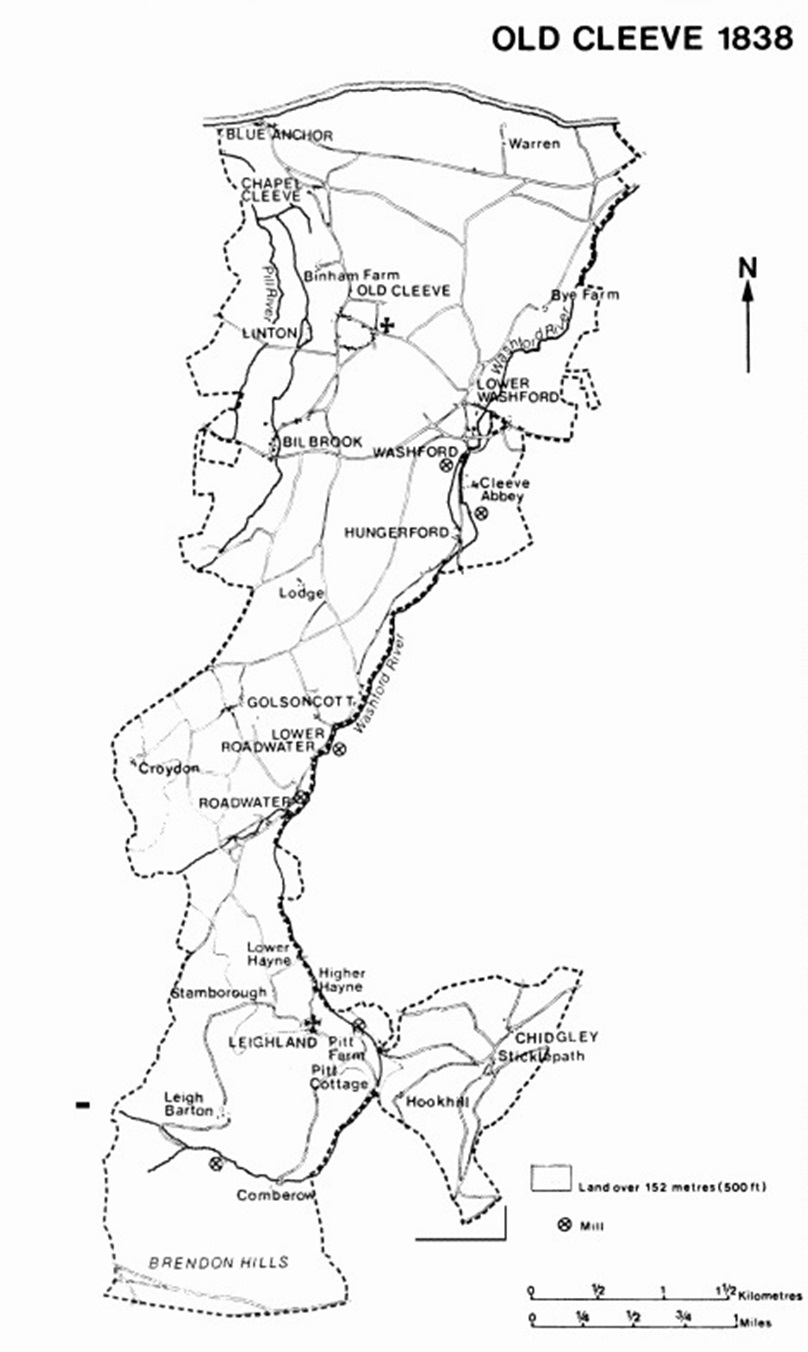
\includegraphics[width=1\textwidth]{figures/oldCleeve}
     \caption{A map of Old Cleeve Parish in 1838}
     \label{fig:OldCleeve}
\end{figure}
 
Little enough room for the energies of vigorous characters to have play, one might think; but surprisingly ample if the energy is of the mind and spirit, for who knows then to what unexplored recesses of the world such radiant energy can find its way? 

I hope I am not labouring the obvious when I insist on the beauty of the scenery of our parish, the freshness of the "meadows and woodlands, the harmonious lines of the green hillsides, the stately heights of the Brendons on which one's gaze rests in the south, the houses which seem to grow out of the rich soil, and all down along the valley the stream, alive with trout, which hurries rippling and murmuring over its stone to find its way at last in gentle meanders to the pearl-grey sea. Even the monks of the Middle Ages, who too often saw in earthly beauty a snare for the spirit, could not hold out against the charm, and they named the place “Vallis florida”. And even the forces of modern progress- the speculative builder, the county surveyor of his minions, the river board, and the “scientific farmer” – though they have attacked this age-old beauty, have not destroyed it. 

Nature here is on the human scale; the beauty has come from man's unconscious partnership with Nature, and for a thousand years and more they have been getting on pretty well together. In the nineteenth century -and Old Cleeve Parish is unique in the distribution of its people, certainly in West Somerset, and probably in all the rural county -the parish supported a population of fifteen or sixteen hundred, living in three sizeable villages, Old Cleeve, Washford, Roadwater, three hamlets, Bilbrooke, Golsoncott and Leighland, and in more than a score of farms and cottages spread along the strea or upon the hillsides. Industries flourished, yet they did not disturb this delicate balance of economy and beauty, for they derived from the life of the country and served essential not artificial needs. Each was an industry of craftsmen, of smiths, millers, wheelwrights, sawyers, carpenters, cordwainers, harnessmakers, and saddlers, lime burners, charcoal burners. Their methods changed little in five hundred years, and they could never have imagined that their crafts might ever pass into oblivion. Men needed food, food must be grown by farmers, farmers needed gorses: these things could never change.

Justifiably they thought so; the Industrial Revolution which had struck the North of England had left the West practically unscathed; and since West Somerset had no coal, there seemed no reason that the new kind of industry should come and break the mould of their contented days- for contented they were, on the whole, despite the hunger. But come it did, and though in the form it assumed it did not break the mould of village life, it made an indelible impression on the minds of the people. 

Up on Brendon Hills, long out of living memory, the “old men” had mined iron ore. Who they were, no one is certain. Germans in Queen Elizabeth’s time, perhaps, for it is known that German miners brought their skills to other parts of the country, notably Cumberland, and it may be more than coincidence that the German word for “iron”, “Eisen”, is found in the name of one tract of the Brendon range, Eisen Hill.  More likely, though, it was the Romans or the Roman Catholics- for to most of the old country people they were one and the same, and they had interestingly confused ideas on the origins of some of the archaeologic al monuments,; and it was all very, very long ago.

But in the 1840’s, the commercial value of the ore began to be appreciated, when Sir Thomas Lethbridge of Luxborough started to mine black haematite ore (with over fifty percent metallic content) on a small scale on Withiel Hill. To samples of this ore were displayed at the Great Exhibition of 1851. Soon a company was formed, based on Ebbw Vale, and for a quarter of a century mines were being sunk or driven in thirty different sites over hills and three quarters of a million tons were taken out. Miners and their families came from Conrwall, South Wales and the North of England, and new communities sprang into life at Brendon Hill and Gupworthy. Few local men worked in the mines, and the farm labourers’ wage did not rise, but the coming of the miners did bring a modest prosperity to the tradesmen of the valley and to the cottagers with whom they lodged until houses were built for them up on the hills as near as possible to their work.. From two to three hundred were employed in the mines, and it is reasonable to assume that the mining families numbered from six to eight hundred persons; two hundred of whom lived in our parish and in the new village of Brendon Hill.

To this day the spoil heaps are clearly to be seen; and here and there lumps of iron ore can be found; but the haematite was generally of high grade too valuable to waste, and I have a sample, once used as a door stop, the size of a melon, with a noded surface as smooth as if polished by an emery wheel. Many of the workings are flooded, and must hold tens of millions of gallons of water; but others are explores from time to time by cavers, and one of these has brought to me a collection of minerals which is remarkably varied for such a small area as ours.

Stemming directly from this enterprise was another, more vital to the life of the parish, and more exciting - I use that much-abused word advisedly- to my forebears. The mines were, in the strictest sense, marginal to their life; this enterprise was central. It was the "mineral line".

The mine heads are mostly situated at twelve hundred feet above sea level, and the ore had to be carted between six and ten miles to the port of Watchet for shipment to the company’s smelting works in Barry, and the roads the carts had to negotiate were not only execrably rutted but also included Sticklepath Hill, a mile long gradient of one in six. Sometimes they would return from Watchet laden with lime or sand for the farms, but by and large the transport threatened to make the mining economically unattractive when the best veins were exhausted.

Legend has it that the head of the company, Charles Edward Rowcliffe, was so moved by seeing an old horse labouring up Sticklepath that he determined to press for a railway. Immediately the surveyors got to work and a line was marked from Watchet up along the banks of the stream for six miles through Washford, Torre and Roadwater to the foot of the hills at Comberow, and thence up the hillside, continuing along the top at a height of 1200 feet for four miles to Gupworthy. The land was bought, and in July, 1855, the first sod was cut at Roughmoor, half-way between Watchet and Conberow, and the gangs of navvies set to work. 

They made swift progress, for the line as far as Comberow follows the easy natural gradient of the valley; but the leap of eight hundred feet from Comberow to the top of the hill was accomplished in a feat of imaginative daring which, if not unique, was essentially Victorian.

\begin{figure}
	 \centering
     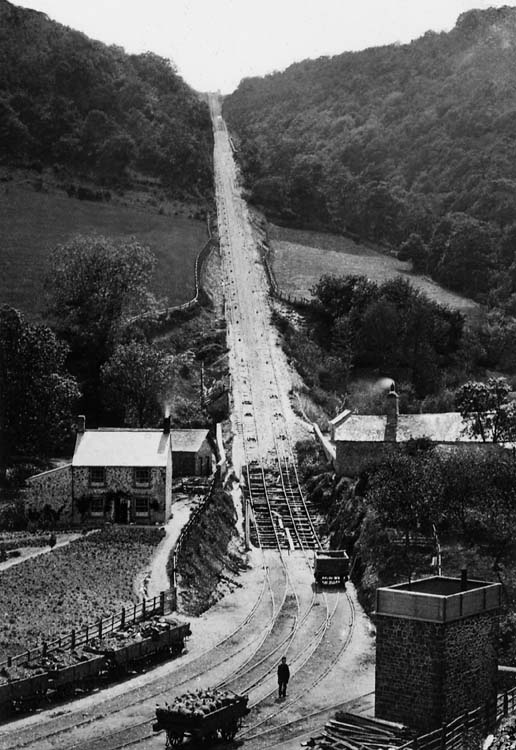
\includegraphics[width=1\textwidth]{figures/comberowIncline}
     \caption{The Incline, Cumberow. Built as part of the West Somerset Mineral Line to transport ore to the port of Watchet}
     \label{fig:Comberow}
\end{figure}

\begin{figure}
	 \centering
     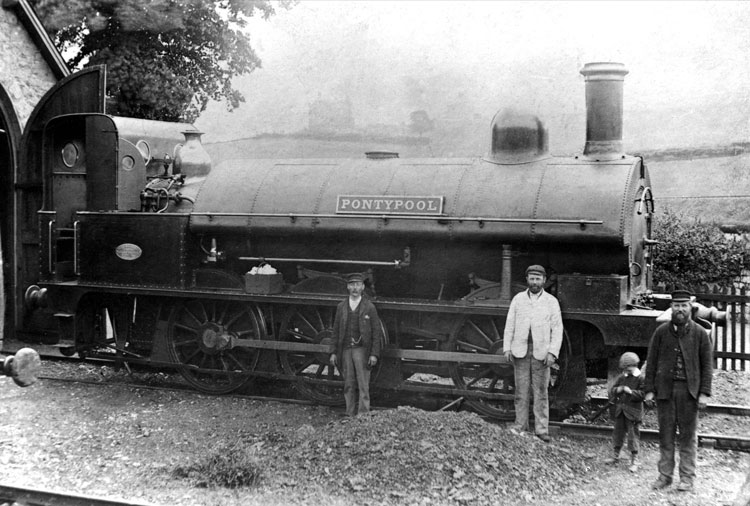
\includegraphics[width=1\textwidth]{figures/pontypoolWatchet}
     \caption{Pontypool at Whitehall shed, Watchet, in 1893}
     \label{fig:Pontypool}
\end{figure}

\begin{figure}
	 \centering
     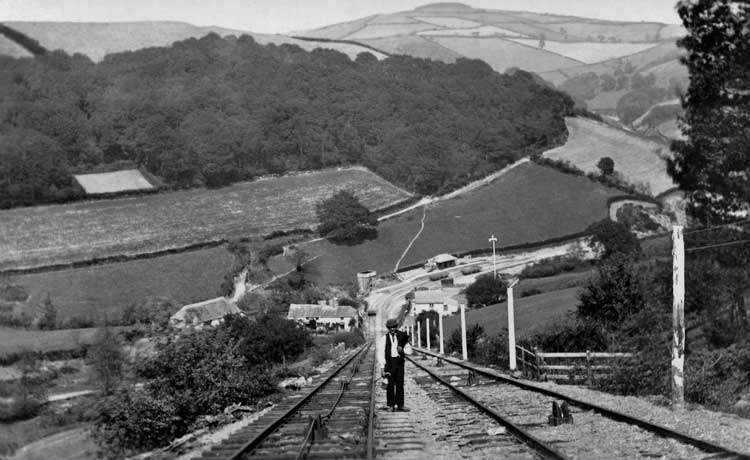
\includegraphics[width=1\textwidth]{figures/inclineTop}
     \caption{A view from Comberow, about one third of the way up the mineral line. Probably taken about 1875, the man, said to be Jack Jewell, stands a little higher upslope than underbridge 14; he carries a can of tallow from lubricating the cable sheaves}
     \label{fig:inclineTop}
\end{figure}

But first I must describe the line as if we were travelling in the "wrong" direction, up from Watchet. For six miles we rise gently enough, pausing at the stations of Washford and Roadwater and the halts of Torre and Clitsome, rarely exceeding a gradient of one on 100 and never straying more than a landyard or two from the bank of the river, until we stop at Comberow, six hundred feet above sea level, in the shadow of the Brendon Hills, where the northern slopes are steepest. We alight and seven hundred feet above us we see the brow of the hill where the mines begin and where we must go. But we stand amazed at what we see: the famous ''Incline”— for the engineer, Rice Hopkins, thrust his railway in double track up. The mountainside at a steady gradient of one in four for three-quarters of a mile. The difficulties were tremendous - outcrops of rock had to be blasted away and depressions filled in, bridges and culverts had to be built, the strictest alignment had to be maintained - but this was the only practicable solution.




My father would say, "You could lay a row of sovereigns end to end from top to bottom of the incline for what it cost the company to build it." It sounds a hyperbole but is literally true at a cost of 180,000 in good Victorian gold, and though the company may have contemplated their bank balance very ruefully they had good cause to be proud of their creation.

One could travel up, at one's own risk, in an open truck, and from the top of the Incline, thirteen hundred feet above sea level, another engine takes you four miles further, over the undulating moorland, to the end of the journey near the mining village of Gupworthy. But the ingenious working of the Incline must be described. It was operated largely by the cheapest and most basic form of power, that of gravity: the weight of a full truck at the top would pull up an empty truck from the bottom; but the speed had to be controlled, and the five thousand foot steel cable joining the trucks was passed round a steel drum eighteen feet high in an engine-house at the top of the incline, and thence down to the lower truck. The full truck with its five tons of ore would be cased over the lip of the incline, and the engine would initially aid it to pull the empty truck at the top of the cable, then as the descending weight increased and the ascending weight diminished, the engine would control the speed. The system worked well and in thirty years of use only two accidents occurred, both from the couplings giving way. In one, a truck loaded with rails broke away when half-way up the Incline, hurling its load of rails into the next field. The other accident - but this has found a place in our family annals and I must duly locate it there.
The coming of the railway to Roadwater threw more than one pebble into the still pond of village life; for a time it brought the "navvies", who no doubt caused some consternation, but it also brought the people of the village into contact with the busy life of Watchet and even - if they could afford it - with the county town of Taunton. Indeed, Roadwater folk were inordinately but understandably proud of having had a railway fifteen years before the pretentious and self-satisfied township of Minehead!

Moreover, the railway came decisively into our family life, for the company built a station at Roadwater, appointed Great-Grandfather Henry as stationmaster and agent, and built him a house. (My maternal grandfather was also a railwayman - a porter, and later inspector, on the Great Western.) Henry was assisted by his younger son William, and William had initiative. When twelve years of age - this must have been in 1859 or 1860 - manning the crossing gates, he heard an unfamiliar noise higher up the valley; moments later, about two hundred yards away, a runaway truck came hurtling round a bend in the track. Without hesitating, young William shut the gates to try to break the speed of the truck, and then ran towards it to escape the flying splinters. The truck of course broke through, and ended its journey in Watchet harbour, but William was commended for his action.
In due course the story acquired the embellishment of a puppy, an involuntary traveller in a closed box left on the truck, which bobbed up to one surface and floated in the harbour until the yelping of its occupant attracted attention and the puppy as saved, none the worse. Whether true or not, it deserves to be.

The mines went well for twenty years, and production rose from 4,000 tons in 1855 to 46,000 in 1877; but in the next year a sharp decline began as ore from Spain was brought in more cheaply. Villages were depopulated almost overnight, and the Brendon Hills found their age-old silences again.

The mining company, under the terms of their Act of Parliament, continued to run the railway for nearly twenty years more, but traffic was generally light, though at times excursions were organised, in connection with the Bible Christian and other chapels at Watchet, Roadwater and Brendon Hill or the flourishing Bands of Hope and Good Templars' Lodge. - But I must say no more of the mines here, for fear of spoiling the fascinating story told, by Roger Sellick and his collaborators in their "West Somerset Mineral Railway".
 
\Flourish 
 
For a hundred yards or so the abandoned Mineral Line runs along the bottom of my garden in Washford. There is little visible record of its history: the rails and sleepers were removed more than half a century ago, and bushes and briars have invaded the track. But if you are keen enough of hearing you will detect, on a still, starlit winter’s night, the sound, of a going in the tops of the alder trees, and if you close your eyes and keep them close, you will hear a soft hiss of escaping steam as an invisible locomotive emerges from the filled-in bridge and glides over the vanished sleepers on its way to Comberow.